\section{Simulation study}

Here we consider inference for a regression parameter $\beta$ of a linear or generalized linear model for a network in the case where there is an omitted variable. The true data-generating models we consider are of the form 

$y_{i,j} \sim  \mu + \beta x_i x_j + \gamma w_i w_j + \epsilon_{i,j} $

where $Y= \{y_{i,j}\}\in \mathbb R^{n\times n}$ is an observed sociomatix, $x = \{x_i \} \in \mathbb R^n$ is a vector of observed node-specific characteristics, and $w = \{ w_i\} \in \mathbb R^n$ is a vector of unobserved node-specific characteristics. We compare inference for $\beta$ using three models:

\begin{itemize}
	\item A naive regression model assuming independent errors; 
	\item A latent factor model; 
	\item An ``oracle'' regression model that includes both $x_{i,j}=x_i x_j$ and $w_{i,j}=w_i w_j$. 
\end{itemize}

We make these comparisons in the context of a binary network outcome with a probit regression model. 

One way to compare inferences across models is  with bias and variance of the parameter estimates. Both of these quantities are combined to get the MSE. 

Alternatively, bias and precision can be summarized by confidence interval coverage and width. Coverage should ideally be at the nominal level. If two methods have the same actual coverage rate, the one with the narrower intervals is preferred. 

\begin{figure}
	\centering
	\caption{Bias in parameter when homophily is ignored.}
	\label{fig:ameBias}
	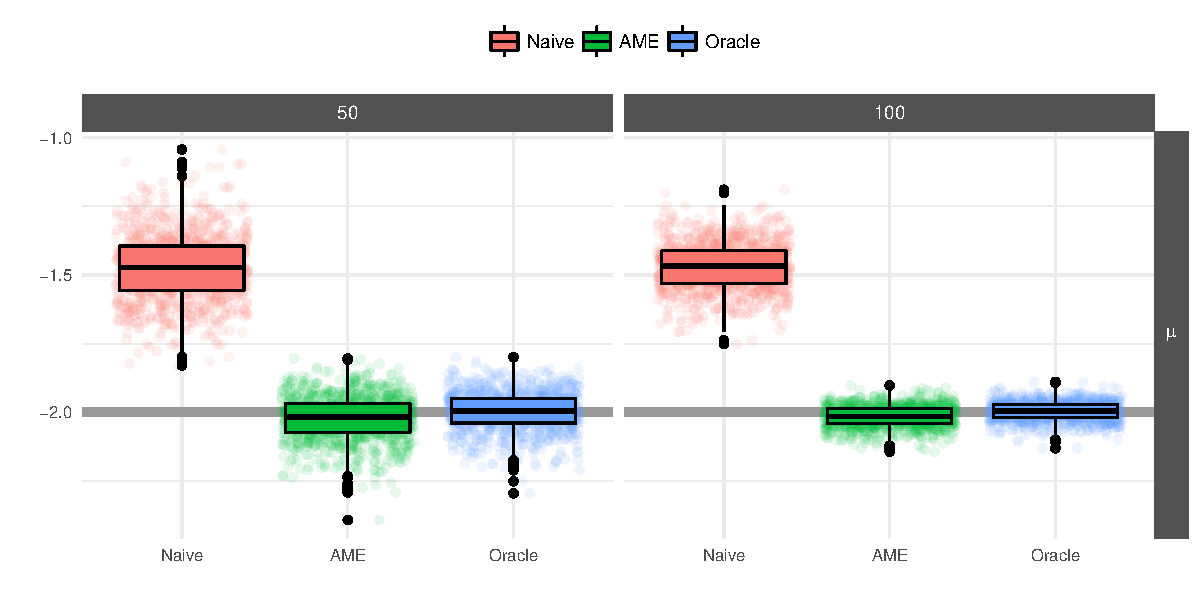
\includegraphics[width=1\textwidth]{ameSimBias_mu.pdf} \\
	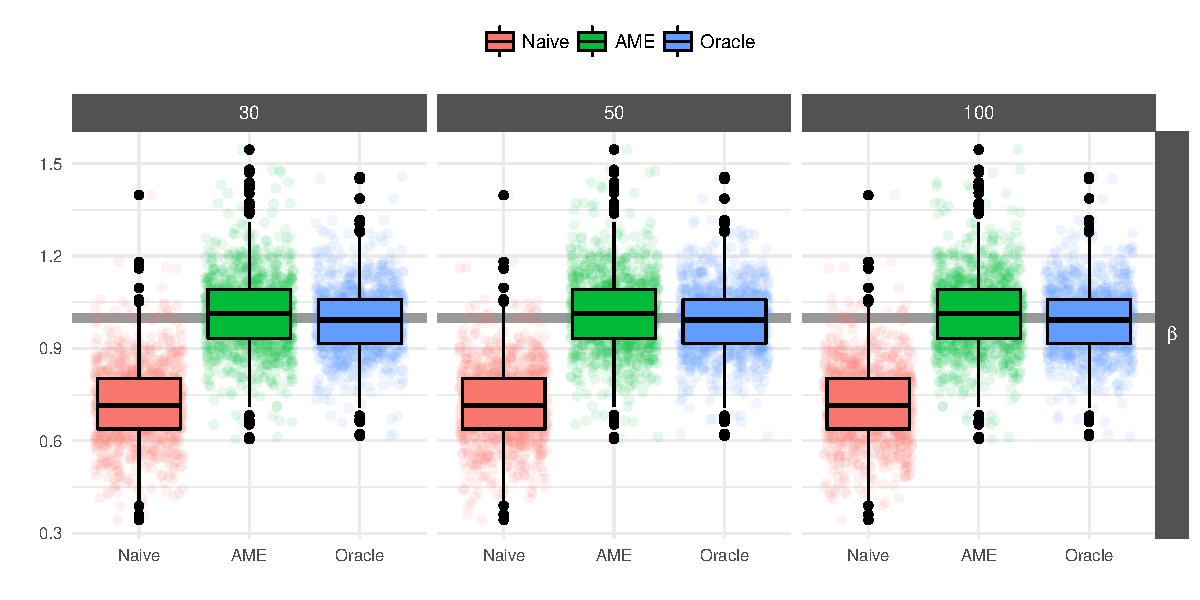
\includegraphics[width=1\textwidth]{ameSimBias_beta.pdf}
\end{figure}

\begin{figure}
	\centering
	\caption{Coverage in parameter when homophily is ignored.}
	\label{fig:ameCalib}
	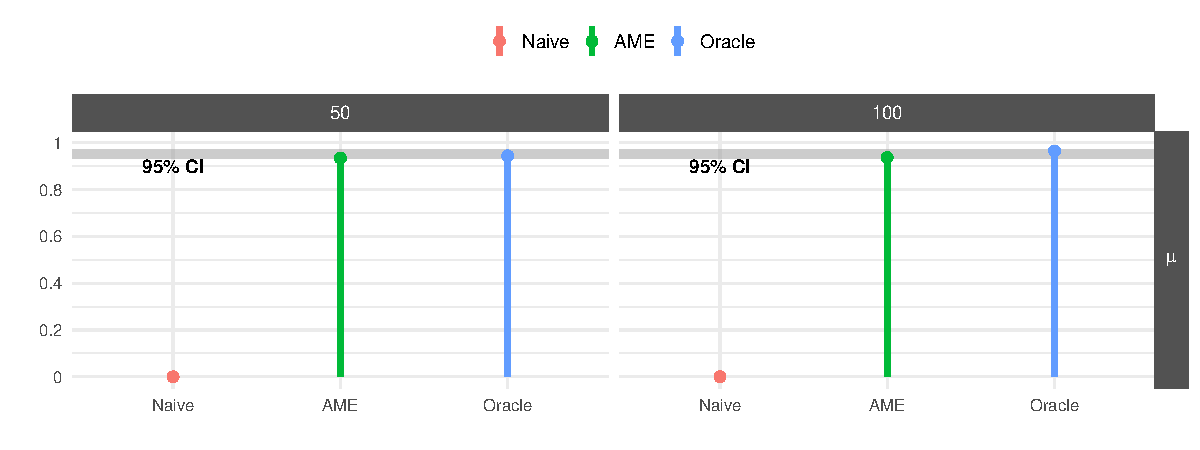
\includegraphics[width=1\textwidth]{ameSimCover_mu.pdf} \\
	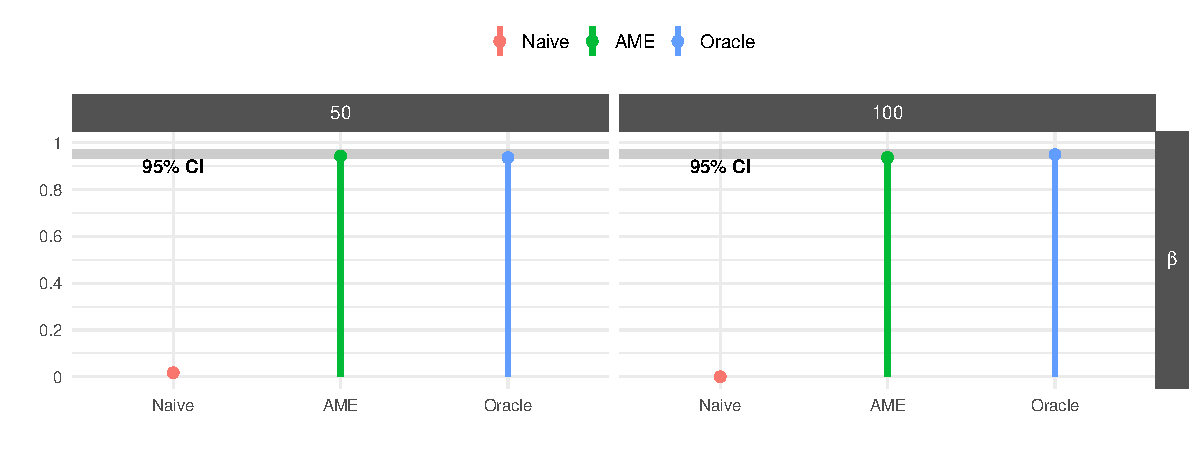
\includegraphics[width=1\textwidth]{ameSimCover_beta.pdf}
\end{figure}

\begin{figure}
	\centering
	\caption{Correlation between missing variable and multiplicative random effect in AME.}
	\label{fig:ameCorr}
	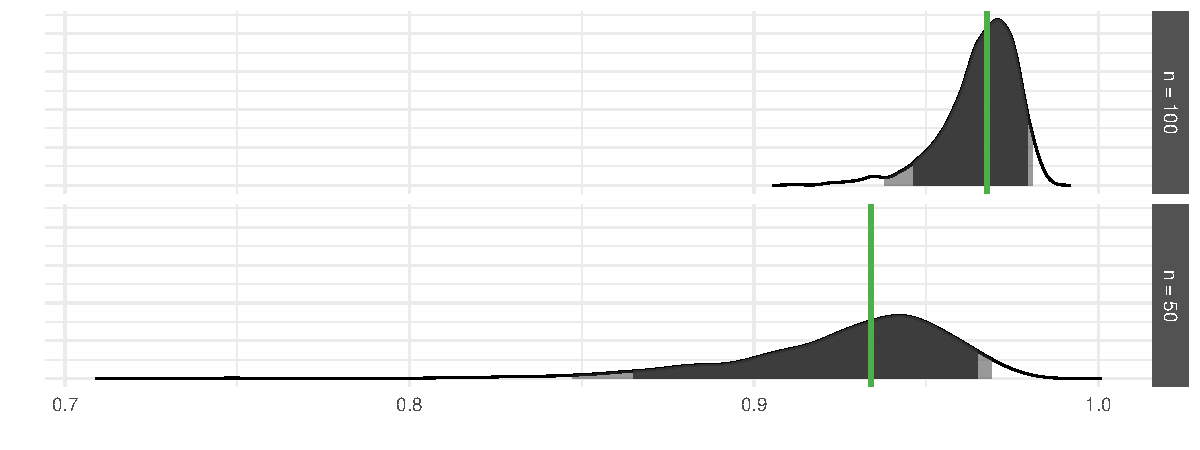
\includegraphics[width=1\textwidth]{ameSimCorr.pdf} \\
\end{figure}
